\renewcommand{\sectiontitle}{Sequencing within intervals}
\section{\sectiontitle}
\customToC{currentsection,hideothersubsections}{}

\begin{frame}{\sectiontitle}
    \begin{itemize}
        \itemj Ejemplar genérico: Un conjunto finito $T$ de tareas y por cada $t\in T$, un entero \textit{tiempo de liberación} $r(t)\geqslant 0$, un \textit{tiempo limite} $d(t)\in \mathrm{Z}^+$ y una longitud $l(t)\in \mathrm{Z}^+$.
        
        \item Pregunta de decisión: ¿Existe un horario factible para $T$, una función $\sigma:T\to \mathrm{Z}^+$ tal que para cada $t\in T$, $\sigma(t)\geqslant r(t), \sigma(t) + l(t)\leqslant d(t)$ y si $t'\in T-\{t\}$ entonces $\sigma(t')+l(t') \leqslant \sigma(t)$ o $\sigma(t') \geqslant \sigma(t) + l(t)$ ?\\
        (la tarea $t$ es ejecutada desde el tiempo $\sigma(t)$ al tiempo $\sigma(t) + l(t)$, no se puede ejecutar hasta el tiempo $r(t)$, debe ser completada para el tiempo $d(t)$ y su ejecución no puede traslaparse con la ejecución de otra tarea $t'$).
    \end{itemize}
\end{frame}

\renewcommand{\subsectiontitle}{Algoritmo no determinista}
\subsection{\subsectiontitle}

\begin{frame}{\subsectiontitle}
    \begin{itemize}
    \itemj Fase Adivinadora\\
    \begin{itemize}
        \item Tiramos un dado equilibrado de $|T|$ lados y del número $n$ que salga tomamos la tarea $t_n$ del conjunto $T$, la renombramos como $t_1'$ hacemos su horario factible igual a $\sigma(t_1')=0$ volvemos a tirar el dado y del número $m$ que salga tomamos la tarea $t_m$ del conjunto $T$, y la renombramos como $t_2'$, hacemos el $\sigma (t_2') = \sigma(t_1') + l(t_1')$, ..., volvemos a tirar el dado y del número $j$ que salga tomamos la tarea $t_j$ del conjunto $T$, y la renombramos como $t_i'$, tal que $t_{i-1}'$ sea la tarea anterior a la que le asignamos su horario factible, hacemos el $\sigma (t_i') = \sigma(t_{i-1}') + l(t_{i-1}')$, y hacemos esto hasta asignarle un horario factible a la tarea $t_{|T|}$.
    \end{itemize}
    
    \item Fase Verificadora\\
    \begin{itemize}
        \item Por cada tarea verificamos que $\sigma(t)\geqslant r(t), \sigma(t) + l(t)\leqslant d(t)$ y si $t'\in T-\{t\}$ entonces $\sigma(t')+l(t') \leqslant \sigma(t)$ o $\sigma(t') \geqslant \sigma(t) + l(t)$, si se cumple para todas las tareas devolvemos SI, en otro caso regresamos NO.
    \end{itemize}
    
    
\end{itemize}
\end{frame}

\renewcommand{\subsectiontitle}{Teorema y Demostración}
\subsection{\subsectiontitle}
% \customToC{currentsection,hideothersubsections}{}

\begin{frame}{\subsectiontitle}
    \begin{itemize}
        \itemj Teorema: El problema secuenciación dentro de intervalos es NP-Completo.
        \item Demostración: Transformamos partición a secuenciación dentro de intervalos.
        \item Para demostrar el problema usaremos la técnica de reemplazo local. Pero primero ¿qué es el problema de partición?
    \end{itemize}
\end{frame}

\renewcommand{\subsectiontitle}{Partición}
\subsection{\subsectiontitle}

\begin{frame}{\subsectiontitle}
    \begin{itemize}
        \itemj Ejemplar genérico: Un multiconjunto $S$ de enteros positivos.
        \item Pregunta de decisión: Existen 2 subconjuntos $S_1$ y $S_2$ tal que la suma de los enteros de $S_1$ sea igual a la suma de los enteros de $S_2$?
        \item Ejemplo:
        Supongamos que tenemos $S=\{3,1,1,2,2,1\}$.\\
        Sea $S_1=\{1,1,1,2\}$ y $S_2=\{2,3\}$ vemos que ambos subconjuntos suman 5 y devuelven YES a la pregunta de decisión. Podemos ver que otra partición la tenemos con los subconjuntos $S_1=\{3,1,1\}$ y $S_2=\{2,2,1\}$ vemos que ambos subconjuntos suman 5.
        \item Dato curioso: Este problema es llamado el problema difícil más fácil.
    \end{itemize}
\end{frame}

\renewcommand{\subsectiontitle}{Transformación}
\subsection{\subsectiontitle}

\begin{frame}{\subsectiontitle}
    \begin{itemize}
        \itemj Sea el conjunto finito $A$ y un tamaño $s(a)$ para cada $a\in A$ el ejemplar genérico del problema partición y $B=\Sigma_{_{a\in A}}$ $ s(a)$.
        \item Las unidades básicas del ejemplar de partición son los elementos individuales $a\in A$.
        \item El reemplazo local para cada $a\in A$ es una sola tarea $t_a$ con $r(t_a)= 0$, $d(t_a)=B+1$ y $l(t_a)=s(a)$. El ejecutor es una sola tarea $\bar{t}$ con $r(\bar{t})= \lceil B/2\rceil$, $d(\bar{t})=\lceil (B+1)/2\rceil$ y $l(\bar{t})=1$.
    \end{itemize}
\end{frame}
\begin{frame}{Complejidad en tiempo de la transformación}
    Claramente este ejemplo puede ser construido en tiempo polinomial desde el ejemplar de partición.
    \begin{itemize}
        \itemj Tomar cada elemento $a\in A$ y asignarle un valor $r(t_a)= 0$, $d(t_a)=B+1$ y $l(t_a)=s(a)$ tiene una complejidad $O(3|A|)$, junto con la generación de la tarea $\bar{t}$ tenemos que la complejidad en tiempo para esta transformación es de tiempo $O(3(|A| +1))$.
    \end{itemize}
\end{frame}

\begin{frame}{Restricciones por $\bar{t}$}
    \begin{itemize}
        \itemj $\bar{t}$ nos asegura que el horario factible no puede ser construido cuando $B$ es un número impar, porque tendríamos que $r(\bar{t})= d(\bar{t})$. Supongamos que $B=3$ entonces $r(\bar{t})= \lceil 3/2\rceil, d(\bar{t})=\lceil (3+1)/2\rceil => r(\bar{t})= \lceil 1.5\rceil, d(\bar{t})=\lceil 4/2\rceil=> r(\bar{t})= 2, d(\bar{t})=2$ y $\bar{t}$ no puede ser agendada. Así que asumimos que $B$ es par.
        \item La segunda restricción la tenemos, ya que $B$ es par, $r(\bar{t})= B/2$ y $d(\bar{t})=r(\bar{t}) +1$, así que algún horario factible debe tener $\sigma(\bar{t})=B/2$. Esto divide el tiempo disponible para agendar las tareas restantes en dos bloques separados, cada uno con longitud de $B/2$ como vemos en la siguiente imagen:
    \end{itemize}
\end{frame}

\begin{frame}
    \begin{figure}
    \centering
        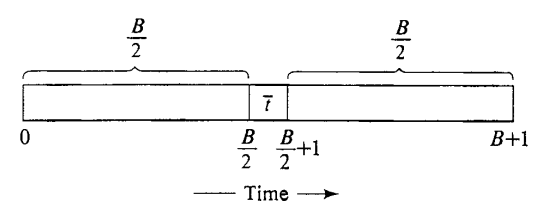
\includegraphics[width=.7\textwidth]{imgs/SWI/SWIdivision.png}
    \end{figure}
    Así el problema de agendación se convierte es un problema de elegir subconjuntos, los que son agendados antes de $\bar{t}$ y los que son agendados después de $\bar{t}$.
\end{frame}

\begin{frame}{Partición = YES =$>$ SWI = YES}
    \begin{itemize}
        \itemj Como la cantidad total de tiempo disponible en los dos bloques es igual al total de la longitud $B$ de las tareas restantes, tenemos que llenar cada bloque de forma exacta.
        \item Esto puede hacerse si y solo si hay un subconjunto $A'\subseteq A$ tal que
        \begin{align*}
            \sum_{a\in A'} s(a) = B/2 = \sum_{a\in A-A'} s(a)
        \end{align*}
        \item Así el subconjunto $A'$ deseado existe para el ejemplar de partición si y solo si existe un horario factible para el ejemplar correspondiente de secuenciación dentro de intervalos.
    \end{itemize}
\end{frame}

\renewcommand{\subsectiontitle}{Ejemplo de transformación}
\subsection{\subsectiontitle}

\begin{frame}{\subsectiontitle}
    Sea $A=\{a_1,a_2,a_3,a_4,a_5,a_6\}$ con $s(a_1)=1,s(a_2)=1,s(a_3)=2,s(a_4)=3,s(a_5)=3,s(a_6)=4$, tenemos que $B=\sum_{1<i<6} s(a_i) = 14$.
    \begin{itemize}
        \itemj Asignamos los valores $r(t_a)=0, d(t_a)=B+1, l(t_a)=s(a)$ para cada $a\in A$:
        
        \vspace{10pt}
        \begin{itemize}
            \item $r(t_{a_1})=0,$ \hspace{5pt} $d(t_{a_1})=B+1=15,$ \hspace{5pt} $l(t_{a_1})=s(a_1)=1$
            \item $r(t_{a_2})=0,$ \hspace{5pt} $d(t_{a_2})=B+1=15,$ \hspace{5pt} $l(t_{a_2})=s(a_2)=1$
            \item $r(t_{a_3})=0,$ \hspace{5pt} $d(t_{a_3})=B+1=15,$ \hspace{5pt} $l(t_{a_3})=s(a_3)=2$
            \item $r(t_{a_4})=0,$ \hspace{5pt} $d(t_{a_4})=B+1=15,$ \hspace{5pt} $l(t_{a_4})=s(a_4)=3$
            \item $r(t_{a_5})=0,$ \hspace{5pt} $d(t_{a_5})=B+1=15,$ \hspace{5pt} $l(t_{a_5})=s(a_5)=3$
            \item $r(t_{a_6})=0,$ \hspace{5pt} $d(t_{a_6})=B+1=15,$ \hspace{5pt} $l(t_{a_6})=s(a_6)=4$
        \end{itemize}

        \item Agregamos la tarea $\bar{t}$  con $r(\bar{t})= \lceil B/2\rceil = \lceil 14/2\rceil = 7$, $d(\bar{t})=\lceil (B+1)/2\rceil=\lceil (14+1)/2\rceil=\lceil 15/2\rceil=\lceil 7.5\rceil = 8$ y $l(\bar{t})=1$.
    \end{itemize}
\end{frame}
\begin{frame}{\subsectiontitle}
    \begin{figure}
    \centering
        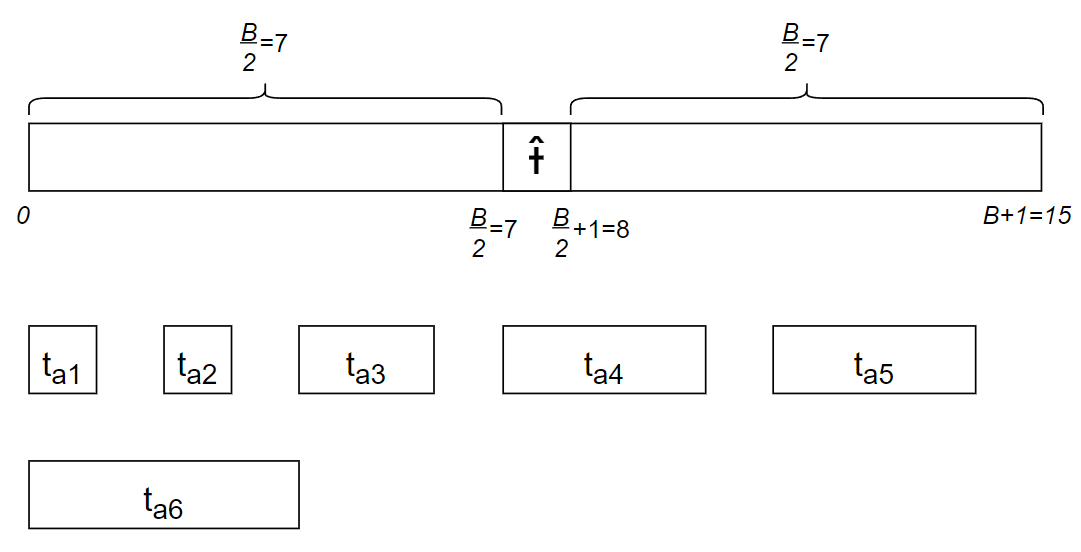
\includegraphics[width=1\textwidth]{imgs/SWI/EjemploSWI_1.png}
    \end{figure}
\end{frame}

\begin{frame}{\subsectiontitle}
    Elegimos el subconjunto $A'=\{a_2,a_3,a_6\}$ y tenemos que $A-A'=\{a_1,a_4,a_5\}$
    \begin{figure}
    \centering
        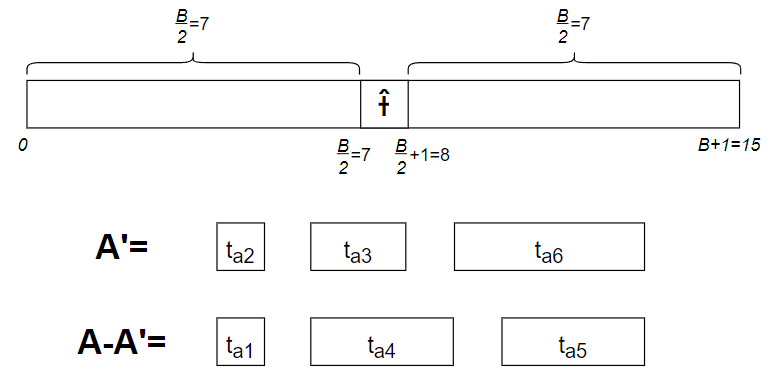
\includegraphics[width=.8\textwidth]{imgs/SWI/EjemploSWI_1_5.png}
    \end{figure}
\end{frame}

\begin{frame}{\subsectiontitle}
    \begin{figure}
    \centering
        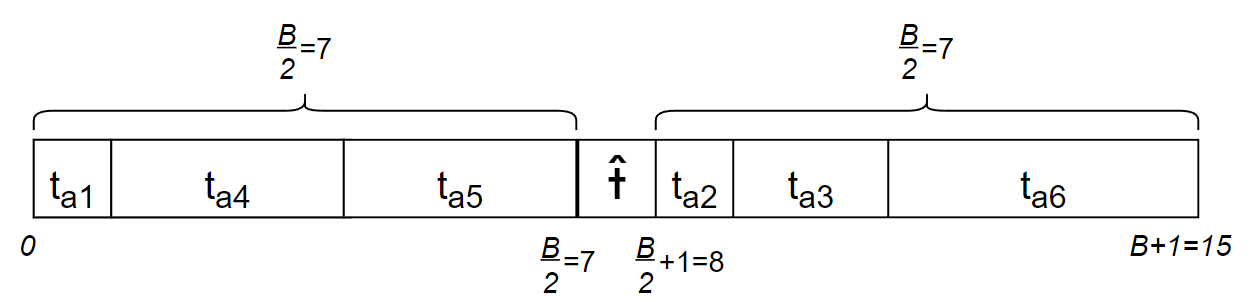
\includegraphics[width=1\textwidth]{imgs/SWI/EjemploSWI_2.png}
    \end{figure}
\end{frame}

\begin{frame}{Aplicaciones en la vida real}
    \begin{itemize}
        \itemj Agendar las tareas que debe realizar una maquina.
        \item Crear horarios bonitos para la escuela.
    \end{itemize}
\end{frame}